% Rapatrié depuis le doc de travail (onglet Article FR), révision 144.

\section{Introduction}
\label{sec:1}

Les chaînes logistiques sont exposées à des perturbations dont les effets durent plusieurs semaines : défaillances de fournisseurs, coupures de liaisons de transport, fermetures de sites, pics de demande ou congestion généralisée. Leurs conséquences économiques, ventes perdues, pénalités contractuelles, transports d'urgence et heures supplémentaires, dépendent non seulement de la sévérité du choc, mais aussi de la rapidité et de la pertinence de la réaction des gestionnaires \citep{sheffi2005book,ivanov2019ijpr}. La robustesse, capacité à absorber un choc sans dégradation, ne suffit donc pas ; la résilience, capacité à limiter la perte et à se rétablir, dépend largement des décisions prises pendant la crise.

La littérature offre une typologie riche des stratégies d'atténuation et de contingence \citep{tomlin2006,chopra2004} et une représentation bien établie de la résilience sous forme de courbe de perte et de rétablissement, le triangle de résilience \citep{bruneau2003}. Les gestionnaires manquent pourtant d'outils d'aide à la décision capables de répondre à deux questions pratiques : face à une perturbation donnée, quelle politique de réaction a le plus de chances d'atteindre un niveau de résilience visé, et, après un rétablissement médiocre, était-ce le choc, le réseau ou la réaction qui était en cause ? Y répondre exige des observations reliant une perturbation, les décisions prises et la trajectoire de performance qui en résulte. De telles données sont rares : les données d'entreprise sont confidentielles et incomplètes, les bases publiques décrivent les perturbations à un niveau macroéconomique sans les décisions, et les études par simulation ne rapportent qu'un petit nombre de cas agrégés \citep{ramzy2022,do2024}.

Cet article propose une démarche en trois étapes pour combler ce manque (Fig.~\ref{fig:d1}). La première génère par simulation des scénarios de crise étiquetés. Un réseau logistique multi-échelon, par exemple le réseau d'origine du jumeau numérique ouvert ISOMORPH \citep{zhang2026isomorph}, représenté par ses seules capacités ou avec ses délais et ses stocks, est soumis à des perturbations maîtrisées, un gestionnaire simulé y réagit, et chaque crise est rejouée sans réaction et sous trois profils de gestionnaire. La deuxième caractérise chaque trajectoire journalière de service par l'ajustement d'une courbe de résilience à sept paramètres et en déduit six indicateurs de résilience. La troisième apprend, à partir de la base obtenue, un réseau bayésien causal \citep{pearl2009} qui permet le pronostic, le diagnostic et la préconisation de politiques de gestion.

\begin{figure*}[htbp]
\centering
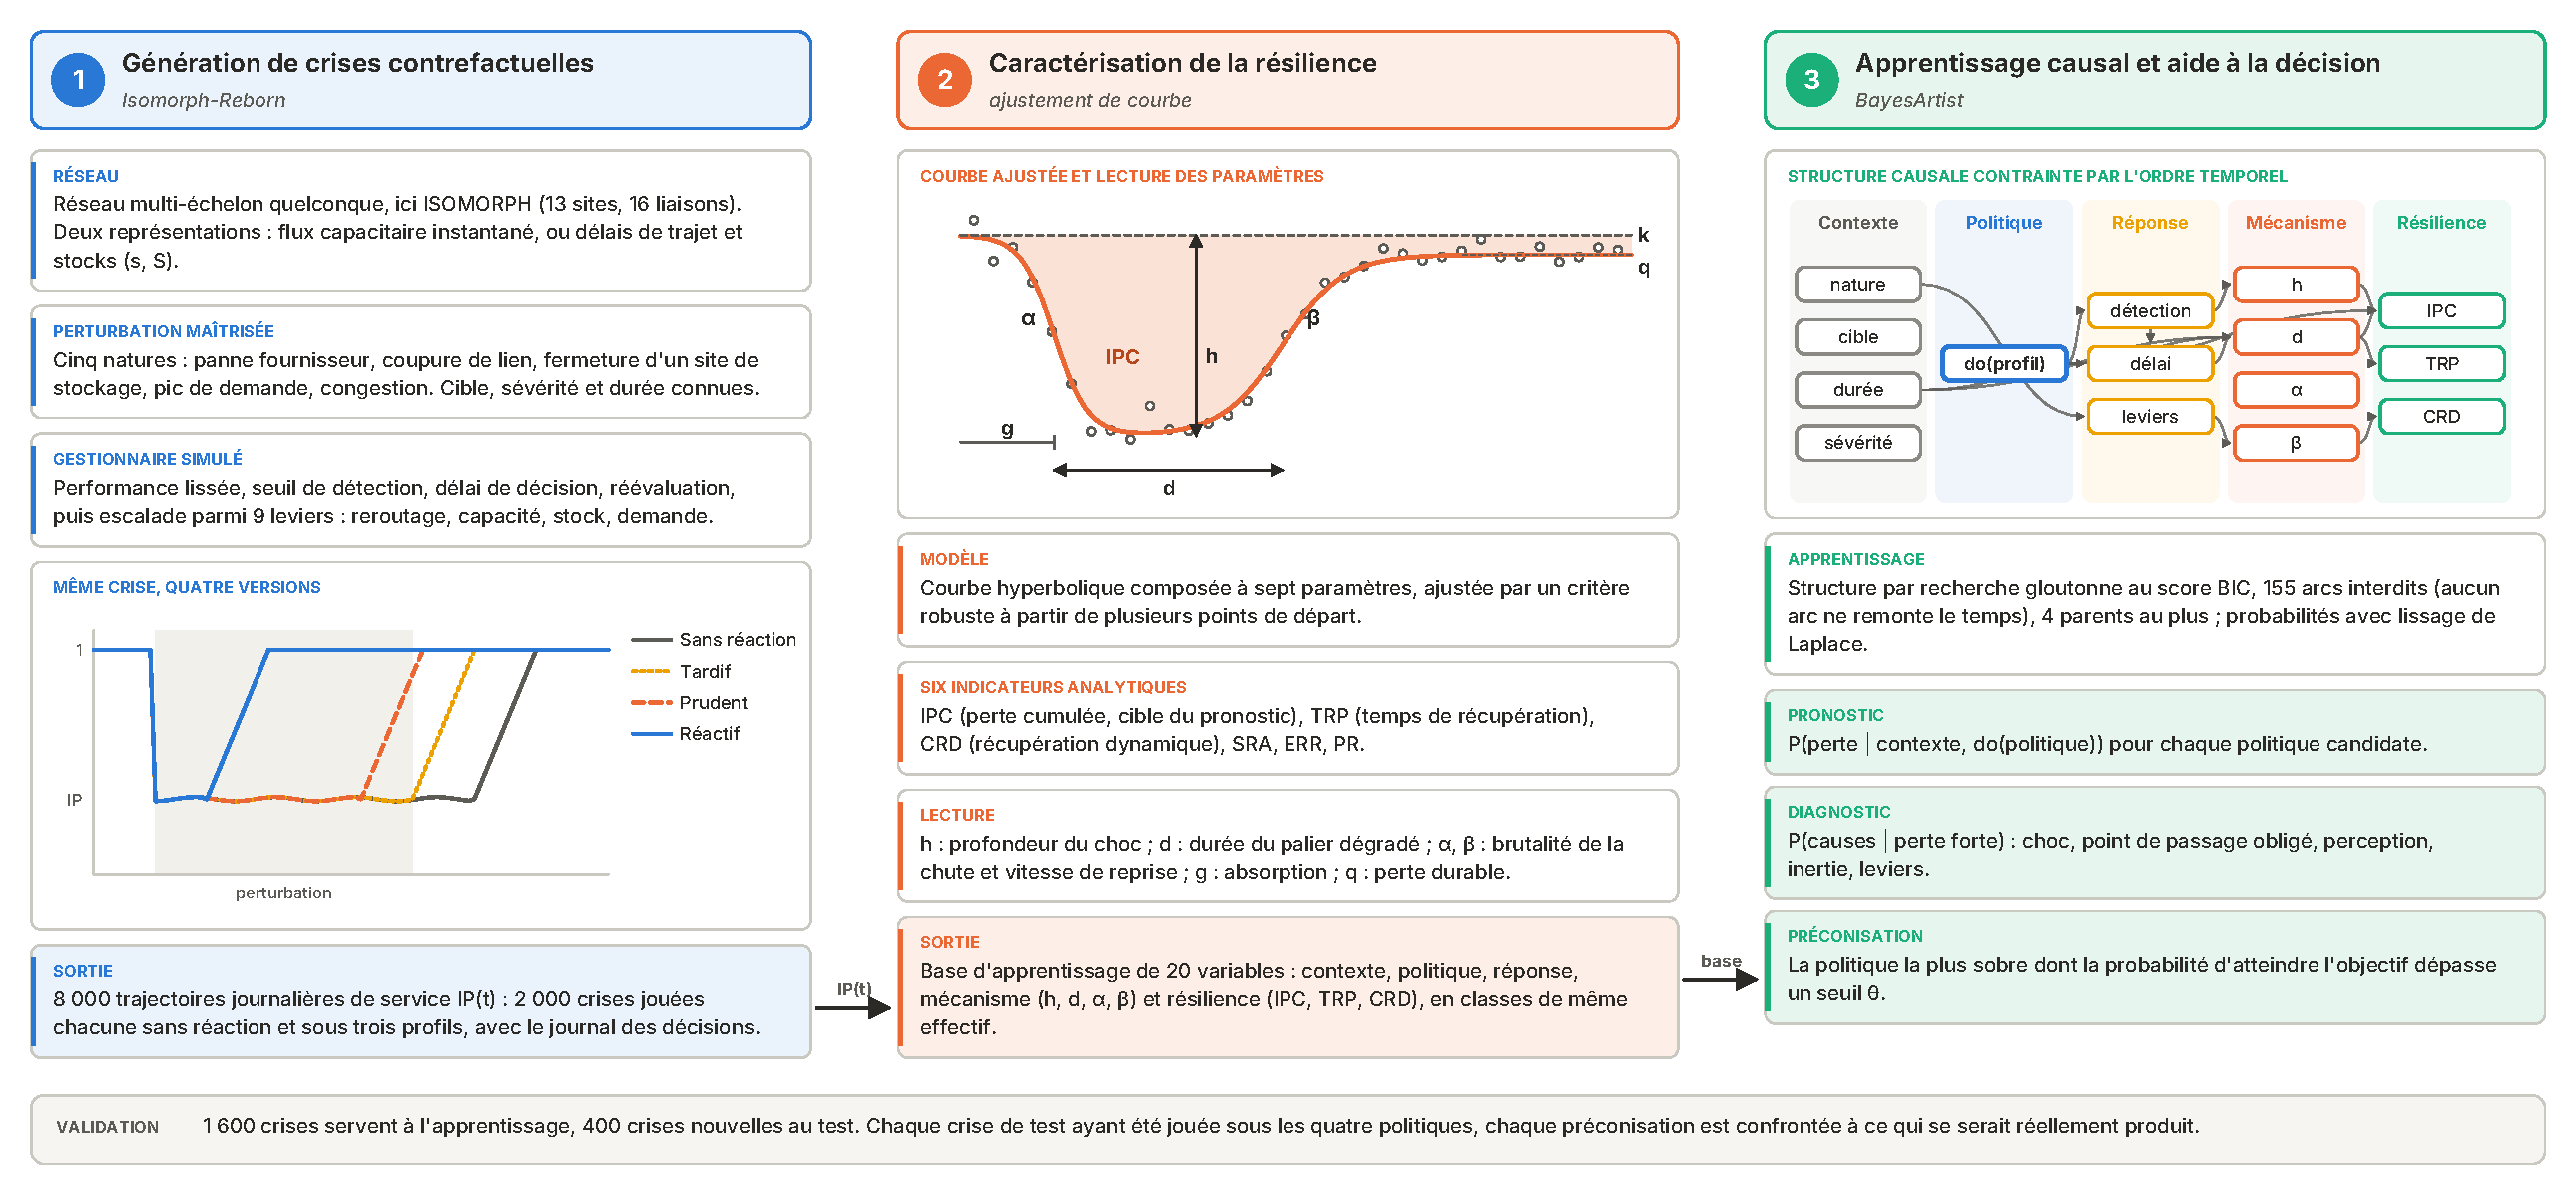
\includegraphics[width=\textwidth]{figures/Fig1_demarche.pdf}
\caption{Démarche en trois blocs. Le bloc 1 joue chaque crise sous quatre politiques de gestion ; le bloc 2 résume chaque trajectoire par une courbe à sept paramètres et six indicateurs ; le bloc 3 apprend un réseau bayésien dont la structure respecte l'ordre temporel d'une crise, et en tire pronostic, diagnostic et préconisation.}
\label{fig:d1}
\end{figure*}

La contribution est triple. D'abord, un générateur de scénarios produisant des crises étiquetées par leur cause exacte et rejouées de manière contrefactuelle, ce qui sépare l'effet de la gestion de celui de la perturbation ; applicable à un réseau multi-échelon quelconque, il fait de la couverture de stock un facteur d'étude plutôt qu'un obstacle. Ensuite, une caractérisation paramétrique de la résilience dont les paramètres ont une lecture opérationnelle directe, reliant la forme d'une crise aux mécanismes de dysfonctionnement. Enfin, un modèle causal dont la structure suit l'ordre temporel d'une crise et traite la politique de gestion comme une intervention, ce qui rend son effet sur la résilience identifiable.

La suite de l'article est organisée comme suit. La section 2 présente l'état de l'art. Les sections 3, 4 et 5 décrivent les trois étapes de la démarche. La section 6 présente les résultats, la section 7 discute les apports, les implications managériales et les limites, et la section 8 conclut.
